\documentclass{article}
\usepackage{amsfonts}
\usepackage{amsmath}
\usepackage{amssymb}
\usepackage{geometry}
\usepackage{hyperref}
\usepackage{pgfplots}
\usepackage{xparse}
\usetikzlibrary{shapes,matrix}
\geometry{margin=1.1in}
\hypersetup{
  colorlinks,
  citecolor=black,
  filecolor=black,
  linkcolor=black,
  urlcolor=black
}
\pgfplotsset{compat=1.9}
\setcounter{secnumdepth}{2}
\setcounter{tocdepth}{1}
\title{%
  When is Phase Modulation (PM) synthesis equivalent to
  Frequency Modulation (FM) synthesis,
  and when do they differ?
}
\author{Attila M. Magyar}
\begin{document}
\maketitle
\tableofcontents

\newpage

  \section{Oscillator Basics}

    The signal generated by an oscillator can be modeled as a function of time
    $O(t)$ where $t$ denotes time, and $O \colon \mathbb{R} \to \mathbb{R}$.

    An oscillator has a waveform associated with it which determines the shape
    of the signal. A waveform is a periodic function; for example, in the
    simplest case, it can be the good old trigonometric sine function. A bare
    $O(t) = \sin(t)$ signal can be thought of as a wave which oscillates once
    every $2\pi$ seconds.

    \begin{figure}[!htb]
      \centering
      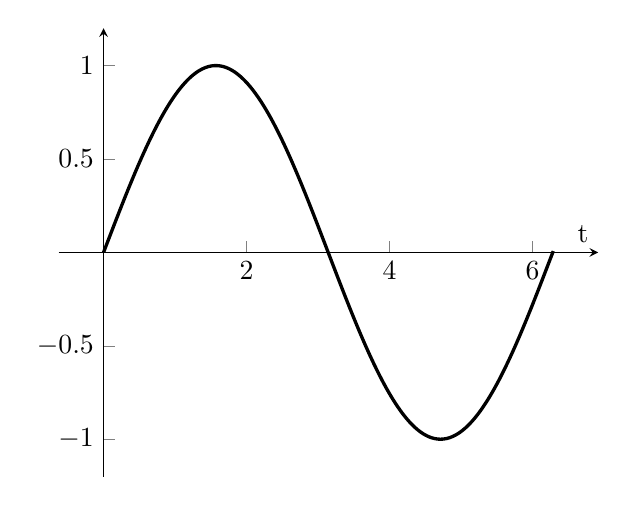
\begin{tikzpicture}
        \begin{axis}[
          axis lines=center,
          enlargelimits,
          tick align=inside,
          domain=0:6.29,
          samples=200,
          xlabel=t,
        ]
          \addplot +[mark=none, line width=1.2, color=black, domain=0:6.29] {sin(deg(\x))};
        \end{axis}
      \end{tikzpicture}
      \caption{%
        Plot of $O(t) = \sin(t)$.
      }
    \end{figure}

    To make it oscillate once every second instead (ie. at 1 Hz), its input
    needs to be scaled by $2\pi$:

    \begin{equation}
      O(t) = \sin(2\pi \cdot t)
    \end{equation}

    \begin{figure}[!htb]
      \centering
      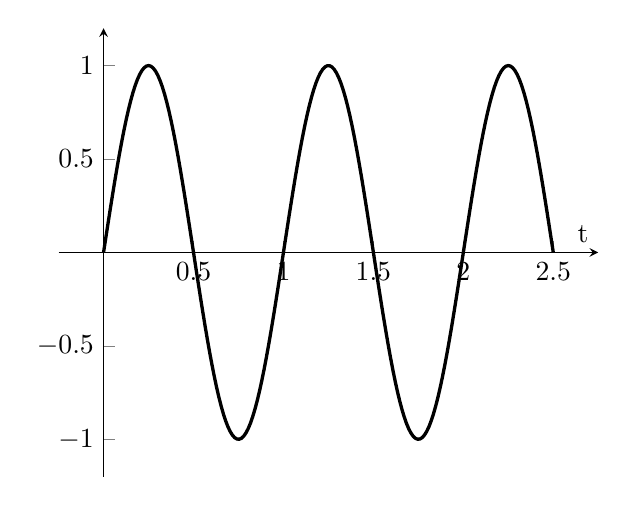
\begin{tikzpicture}
        \begin{axis}[
          axis lines=center,
          enlargelimits,
          tick align=inside,
          domain=0:2.5,
          samples=200,
          xlabel=t,
        ]
          \addplot +[mark=none, line width=1.2, color=black, domain=0:2.5] {sin(2*3.1415*deg(\x))};
        \end{axis}
      \end{tikzpicture}
      \caption{%
        Plot of $O(t) = \sin(2\pi \cdot t)$.
      }
    \end{figure}

    To make it oscillate 3 times per second (ie. at 3 Hz), the input needs to be
    scaled even more:

    \begin{equation}
      O(t) = \sin(2\pi \cdot 3 \cdot t)
    \end{equation}

    \begin{figure}[!htb]
      \centering
      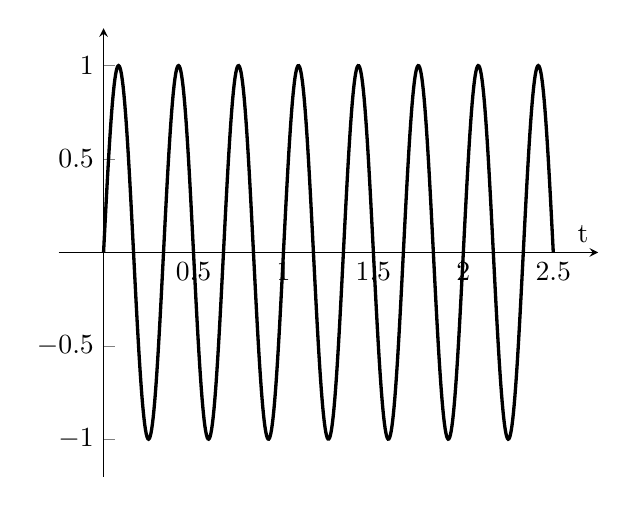
\begin{tikzpicture}
        \begin{axis}[
          axis lines=center,
          enlargelimits,
          tick align=inside,
          domain=0:2.5,
          samples=600,
          xlabel=t,
        ]
          \addplot +[mark=none, line width=1.2, color=black, domain=0:2.5] {sin(2*3.1415*3*deg(\x))};
        \end{axis}
      \end{tikzpicture}
      \caption{%
        Plot of $O(t) = \sin(2\pi \cdot 3 \cdot t)$.
      }
    \end{figure}

    To make it oscillate at a constant frequency $f$, the input needs to be
    scaled by $f$:

    \begin{equation}
      O(t) = \sin(2\pi \cdot f \cdot t)
    \end{equation}

    To start the signal at a different portion of the sine wave at $t = 0$
    seconds, the input needs to be shifted by some number
    $\varphi \in \mathbb{R}$ which is called the "phase" or "phase offset":

    \begin{equation}
      O(t) = \sin(2\pi \cdot f \cdot t + \varphi)
    \end{equation}

    The signal's amplitude can be changed as well by multiplying the whole thing
    by some number $A \in \mathbb{R}$:

    \begin{equation}
      O(t) = A \cdot \sin(2\pi \cdot f \cdot t + \varphi)
    \end{equation}

    (See also: \url{https://en.wikipedia.org/wiki/Sine\_wave}.)

    But what does $2\pi \cdot f \cdot t + \varphi$ actually represent here?

    The input to the sine function can be thought of as an angle measured in
    radians, hence the $2\pi$ term. Whatever this angle is measuring (e.g. it
    could be the rotation of a tonewheel), seems to be changing over time,
    since we have a time-dependent term in there. The trick is that what the
    frequency is measuring here is the "rate of change" (also known as the "time
    derivative") of this angle, telling how many full rotations are completed
    per second, similarly to how velocity in physics measures how many
    kilometers or miles are traveled per second.

    Therefore $2\pi \cdot f \cdot t + \varphi$ here represents the total
    rotation of \textit{something}, which has accumulated over a time span of
    $t$ seconds. In other words, time and frequency aren't just multiplied
    together here: what's happening actually is that instantaneous changes of
    angle are being summed over a length of time which is divided into
    infinitesimally short intervals. So the equation should really look like
    this:

    \begin{equation}
      O(t) =
        A \cdot \sin \left( 2\pi \cdot \int_{0}^{t} f \  d\tau + \varphi \right)
    \end{equation}

    This isn't just unnecesessary, arbitrary pedantry, because the integration
    actually makes a huge difference when the constant frequency is replaced
    with one that is changing over time, which is necessary for modeling
    frequency modulation that is all about changing the frequency rapidly in
    each moment.

    See also:

    \begin{itemize}
      \item \url{https://en.wikipedia.org/wiki/Radian}
      \item \url{https://en.wikipedia.org/wiki/Tonewheel}
      \item \url{https://en.wikipedia.org/wiki/Time\_derivative}
      \item \url{https://en.wikipedia.org/wiki/Instantaneous\_phase\_and\_frequency}
    \end{itemize}

    So let's replace the constant frequency with a function of time,
    $f \colon \mathbb{R} \to \mathbb{R}$:

    \begin{equation}
      O(t)
        = A \cdot \sin \left(
            2\pi \cdot \int_{0}^{t} f(\tau) \  d\tau + \varphi
          \right)
    \end{equation}

    Finally, $\sin(t)$ can be replaced with some other periodic function
    $W \colon \mathbb{R} \to \mathbb{R}$ in order to get a different waveform
    (like sawtooth, triangle, etc.):

    \begin{equation}\label{eqoscillator}
      O(t)
        = A \cdot W \left(
            2\pi \cdot \int_{0}^{t} f(\tau) \  d\tau + \varphi
          \right)
    \end{equation}

  \section{Modulator and Carrier}

    The simplest case of modulation uses two oscillators: the Modulator and the
    Carrier. These are connected in a way which lets the Modulator affect one
    of the parameters of the Carrier. For example, in each moment in time, the
    momentary signal value of the Modulator is added to the selected parameter
    of the Carrier.

    To see how Phase Modulation (PM) and Frequency Modulation (FM) are related
    to each other, we are going to mathematically model FM, and see if we can
    throw enough algebra at it to turn it into PM, then we will look at what
    happens to the modulator function in the process.

    The signals generated by the two oscillators will be modeled as functions
    of time, similarly to equation \ref{eqoscillator}: $M(t)$ and $C(t)$ for
    the Modulator and the Carrier respectively, where
    $M \colon \mathbb{R} \to \mathbb{R}$ and
    $C \colon \mathbb{R} \to \mathbb{R}$.

    For simplicity's sake, let's define $M(t)$ with a constant frequency
    $f_M \in \mathbb{R}$, and a constant amplitude $A_M \in \mathbb{R}$, with
    zero phase offset ($\varphi_M = 0$), and with a waveform
    $W_M \colon \mathbb{R} \to \mathbb{R}$:

    \begin{equation}\label{eqmodulator}
      \begin{split}
        M(t) = & A_M \cdot W_M(2\pi \cdot f_M \cdot t + \varphi_M) \\
             = & A_M \cdot W_M(2\pi \cdot f_M \cdot t + 0) \\
             = & A_M \cdot W_M(2\pi \cdot f_M \cdot t)
      \end{split}
    \end{equation}

    Now let's define the Carrier's function with varying frequency; similarly
    to the above, $A_C \in \mathbb{R}$ is the amplitude,
    $\varphi_C \in \mathbb{R}$ is the phase offset,
    $f_{FM} \colon \mathbb{R} \to \mathbb{R}$ is the varying frequency, and
    $W_C \colon \mathbb{R} \to \mathbb{R}$ is the waveform:

    \begin{equation}\label{eqcarrier}
      C(t) =
        A_C \cdot W_C \left(
          2\pi \cdot \int_{0}^{t} f_{FM}(\tau) \  d\tau + \varphi_C
        \right)
    \end{equation}

    Let's say that the Carrier's own frequency is a constant
    $f_C \in \mathbb{R}$, and this is what is being modulated with $M$, so
    $f_{FM}(\tau)$ can be expressed as:

    \begin{equation}\label{eqffm}
      f_{FM}(\tau) = M(\tau) + f_C
    \end{equation}

    The fundamental theorem of calculus already seems to suggest that
    modulating the frequency by some function is equivalent to modulating the
    phase by an antiderivative of that function. Though there are special cases
    where those two are equivalent, that is not the general case, as it will be
    shown in the next section.

    (See: \url{https://en.wikipedia.org/wiki/Fundamental\_theorem\_of\_calculus}.)

  \section{Turning FM into PM}

    Substituting equation \ref{eqffm} into equation \ref{eqcarrier} and then
    expanding $M$, we get:

    \begin{equation}\label{eqcexp1}
      \begin{split}
        C(t)
          = & A_C \cdot W_C \left(
                2\pi \cdot \int_{0}^{t} \left( M(\tau) + f_C \right) \  d\tau
                + \varphi_C
              \right) \\
          = & A_C \cdot W_C \left(
                2\pi \cdot \int_{0}^{t} M(\tau) \ d\tau
                + 2\pi \cdot \int_{0}^{t} f_C \  d\tau
                + \varphi_C
              \right) \\
          = & A_C \cdot W_C \left(
                2\pi \cdot \int_{0}^{t}
                    A_M \cdot W_M(2\pi \cdot f_M \cdot \tau)
                \ d\tau
                + 2\pi \cdot f_C \cdot t
                + \varphi_C
              \right) \\
          = & A_C \cdot W_C \left(
                2\pi \cdot A_M \cdot \int_{0}^{t}
                    W_M(2\pi \cdot f_M \cdot \tau)
                \ d\tau
                + 2\pi \cdot f_C \cdot t
                + \varphi_C
              \right)
      \end{split}
    \end{equation}

    Thanks to Fourier, it is known that periodic functions can be expressed as
    sums of sinusoids, so for simplicity's sake, let's consider only those
    waveforms for the Modulator where, for some $N \in \mathbb{N}$, $W_M$ can
    be written as:

    \begin{equation}\label{eqmfur}
      W_M(\tau) = \sum_{n=1}^{N} \left( B_n \cdot \sin(n\tau) \right)
    \end{equation}

    where $B_n \in \mathbb{R}$ are some constants for
    $n \in \mathbb{N}, \  1 \le n \le N$.

    (See: \url{https://en.wikipedia.org/wiki/Fourier\_series})

    Expressing $W_M$ in the integral in equation \ref{eqcexp1} as a sum of
    sines yields:

    \begin{equation}\label{eqcexp2}
      \begin{split}
        \int_{0}^{t} W_M(2\pi \cdot f_M \cdot \tau) \ d\tau
          = & \int_{0}^{t}
                \sum_{n=1}^{N} B_n \cdot \sin(2\pi \cdot f_M \cdot n \cdot \tau)
              \ d\tau \\
          = & \sum_{n=1}^{N}
                B_n \cdot \int_{0}^{t}
                  \sin(2\pi \cdot f_M \cdot n \cdot \tau)
                \ d\tau
      \end{split}
    \end{equation}

    Using the fact that for any constant $0 \neq \gamma \in \mathbb{R}$:

    \begin{equation}
      \int \sin(\gamma x) \ dx = - \frac{1}{\gamma} \cos(\gamma x) + c
    \end{equation}

    where $c \in \mathbb{R}$ is the constant of integration, we can calculate
    the integral in the right side of equation \ref{eqcexp2}:

    \begin{equation}\label{eqcexp3}
      \begin{split}
        \int_{0}^{t} \sin(2\pi \cdot f_M \cdot n \cdot \tau) \ d\tau
          = & \left[
                - \frac{1}{2\pi \cdot f_M \cdot n}
                \cdot \cos(2\pi \cdot f_M \cdot n \cdot \tau)
              \right]_0^t \\
          = & - \frac{1}{2\pi \cdot f_M \cdot n}
              \cdot \left[ \cos(2\pi \cdot f_M \cdot n \cdot \tau) \right]_0^t \\
          = & - \frac{1}{2\pi \cdot f_M \cdot n}
              \cdot (
                \cos(2\pi \cdot f_M \cdot n \cdot t)
                - \cos(2\pi \cdot f_M \cdot n \cdot 0)
              ) \\
          = & - \frac{1}{2\pi \cdot f_M \cdot n} \cdot (
                \cos(2\pi \cdot f_M \cdot n \cdot t) - \cos(0)
              ) \\
          = & - \frac{1}{2\pi \cdot f_M \cdot n} \cdot (
                \cos(2\pi \cdot f_M \cdot n \cdot t) - 1
              ) \\
          = & - \frac{
                \cos(2\pi \cdot f_M \cdot n \cdot t) - 1
              }{2\pi \cdot f_M \cdot n} \\
          = & \frac{
                1 - \cos(2\pi \cdot f_M \cdot n \cdot t)
              }{2\pi \cdot f_M \cdot n}
      \end{split}
    \end{equation}

    Furthermore, since $\sin(x-\frac{\pi}{2}) = -\cos(x)$, the result in
    equation \ref{eqcexp3} can be written as:

    \begin{equation}\label{eqcexp4}
      \int_{0}^{t} \sin(2\pi \cdot f_M \cdot n \cdot \tau) \ d\tau
        = \frac{
            1 + \sin \left( 2\pi \cdot f_M \cdot n \cdot t - \frac{\pi}{2} \right)
        }{2\pi \cdot f_M \cdot n}
    \end{equation}

    Plugging equation \ref{eqcexp4} back into the right side of equation
    \ref{eqcexp2}:

    \begin{equation}\label{eqcexp5}
      \begin{split}
        \sum_{n=1}^{N}
          B_n \cdot \int_{0}^{t} \sin(2\pi \cdot f_M \cdot n \cdot \tau) \ d\tau
            = & \sum_{n=1}^{N}
                  B_n \cdot \frac{1 + \sin \left(
                    2\pi \cdot f_M \cdot n \cdot t - \frac{\pi}{2}
                  \right)}{2\pi \cdot f_M \cdot n} \\
            = & \sum_{n=1}^{N}
                  \frac{B_n}{2\pi \cdot f_M \cdot n}
                  + \frac{1}{2\pi \cdot f_M} \cdot \sum_{n=1}^{N}
                      \frac{B_n}{n} \cdot \sin \left(
                        2\pi \cdot f_M \cdot n \cdot t - \frac{\pi}{2}
                      \right)
      \end{split}
    \end{equation}

    Let's define two more constants, $\alpha \in \mathbb{R}$ and
    $\beta \in \mathbb{R}$:

    \begin{equation}
      \begin{split}
        \alpha = & \sum_{n=1}^{N} \frac{B_n}{2\pi \cdot f_M \cdot n} \\
        \beta = & \frac{1}{2\pi \cdot f_M}
      \end{split}
    \end{equation}

    Now we can rewrite equation \ref{eqcexp5} as:

    \begin{equation}\label{eqcexp6}
      \sum_{n=1}^{N}
        B_n
        \cdot \int_{0}^{t} \sin(2\pi \cdot f_M \cdot n \cdot \tau) \ d\tau
          = \alpha
            + \beta
            \cdot \sum_{n=1}^{N}
              \frac{B_n}{n} \cdot \sin \left(
                2\pi \cdot f_M \cdot n \cdot t - \frac{\pi}{2}
              \right)
    \end{equation}

    Continuing equation \ref{eqcexp2} using equation \ref{eqcexp6}:

    \begin{equation}\label{eqcexp7}
      \begin{split}
        \int_{0}^{t} W_M(2\pi \cdot f_M \cdot \tau) \ d\tau
          = & \ \alpha
              + \beta \cdot \sum_{n=1}^{N}
                  \frac{B_n}{n} \cdot \sin \left(
                    2\pi \cdot f_M \cdot n \cdot t - \frac{\pi}{2}
                  \right)
      \end{split}
    \end{equation}

    By plugging equation \ref{eqcexp7} back into equation \ref{eqcexp1}, we
    obtain:

    \begin{equation}\label{eqcexp8}
      \begin{split}
        C(t)
          = & A_C \cdot W_C \left(
                2\pi \cdot A_M
                \cdot \int_{0}^{t}
                  W_M \left( 2\pi \cdot f_M \cdot \tau \right) \ d\tau
                + 2\pi \cdot f_C \cdot t
                + \varphi_C
              \right) \\
          = & A_C \cdot W_C \left(
                2\pi \cdot A_M \cdot \left(
                  \alpha
                  + \beta \cdot \sum_{n=1}^{N}
                      \frac{B_n}{n}
                      \cdot \sin \left(
                        2\pi \cdot f_M \cdot n \cdot t - \frac{\pi}{2}
                      \right)
                \right)
                + 2\pi \cdot f_C \cdot t
                + \varphi_C
              \right) \\
          = & A_C \cdot W_C \left(
                2\pi \cdot A_M \cdot \alpha
                + 2\pi \cdot A_M \cdot \beta \cdot \sum_{n=1}^{N}
                    \frac{B_n}{n}
                    \cdot \sin \left(
                      2\pi \cdot f_M \cdot n \cdot t - \frac{\pi}{2}
                    \right)
                + 2\pi \cdot f_C \cdot t
                + \varphi_C
              \right) \\
          = & A_C \cdot W_C \left(
                2\pi \cdot f_C \cdot t
                + \varphi_C
                + 2\pi \cdot A_M \cdot \alpha
                + 2\pi \cdot A_M \cdot \beta \cdot \sum_{n=1}^{N}
                    \frac{B_n}{n}
                    \cdot \sin \left(
                      2\pi \cdot f_M \cdot n \cdot t - \frac{\pi}{2}
                    \right)
              \right)
      \end{split}
    \end{equation}

    Finally, we can define two more constants $A_{FM} \in \mathbb{R}$ and
    $\varphi_{FM} \in \mathbb{R}$ as:

    \begin{equation}
      \begin{split}
        A_{FM}
          = & \ 2\pi \cdot A_M \cdot \beta \\
          = & \ 2\pi \cdot A_M \cdot \frac{1}{2\pi \cdot f_M} \\
          = & \frac{A_M}{f_M} \\
        \varphi_{FM}
          = & \ \varphi_C + 2\pi \cdot A_M \cdot \alpha \\
          = & \ \varphi_C
                  + 2\pi \cdot A_M \cdot \sum_{n=1}^{N}
                    \frac{B_n}{2\pi \cdot f_M \cdot n} \\
          = & \ \varphi_C + \frac{A_M}{f_M} \cdot \sum_{n=1}^{N} \frac{B_n}{n}
      \end{split}
    \end{equation}

    With these, equation \ref{eqcexp8} takes the following form:

    \begin{equation}\label{eqcexp9}
      C(t)
        = A_C \cdot W_C \left(
            2\pi \cdot f_C \cdot t
            + \varphi_{FM}
            + A_{FM} \cdot \sum_{n=1}^{N}
                \frac{B_n}{n}
                \cdot \sin \left(
                  2\pi \cdot f_M \cdot n \cdot t - \frac{\pi}{2}
                \right)
          \right)
    \end{equation}

  \section{Conclusion}

    For the special case of $N=1$ in equation \ref{eqmfur}, equation
    \ref{eqcexp9} becomes:

    \begin{equation}\label{eqcexp10}
      \begin{split}
        C(t)
          = & A_C \cdot W_C \left(
                2\pi \cdot f_C \cdot t
                + \varphi_{FM}
                + A_{FM} \cdot B_1 \cdot \sin \left(
                  2\pi \cdot f_M \cdot t - \frac{\pi}{2}
                \right)
              \right) \\
          = & A_C \cdot W_C \left(
                2\pi \cdot f_C \cdot t
                + \varphi_{FM}
                + A_{FM} \cdot W_M \left(
                  2\pi \cdot f_M \cdot t - \frac{\pi}{2}
                \right)
              \right)
      \end{split}
    \end{equation}

    which is indeed the same as if we added a constant offset to $\varphi_C$
    and then modulated it by a slight variation of the original modulator
    signal which would have an amplitude of $A_{FM}$ and a phase offset of
    $- \frac{\pi}{2}$ (see equation \ref{eqmodulator}):

    \begin{equation}
      \begin{split}
        M(t)
          = & A_M \cdot W_M (2\pi \cdot f_M \cdot t + 0) \\
        \hat{M_1}(t)
          = & A_{FM} \cdot W_M \left(
                2\pi \cdot f_M \cdot t - \frac{\pi}{2}
              \right) \\
        C(t)
          = & A_C \cdot W_C \left(
                2\pi \cdot \int_{0}^{t} \left( M(\tau) + f_C \right) \  d\tau
                + \varphi_C
              \right) \\
          = & A_C \cdot W_C \left(
                2\pi \cdot f_C \cdot t + \varphi_{FM} + \hat{M_1}(t)
              \right)
      \end{split}
    \end{equation}

    Therefore for $N = 1$, phase modulation and frequency modulation are indeed
    equivalent sonically with the right choice of amplitude and phase offset.

    But for $N > 1$, if the frequency modulated $C(t)$ signal is expressed as a
    phase modulated signal, as can bee seen from equation \ref{eqcexp9}, we get
    a modulator signal which has a significantly different harmonic content
    from the original $M(t)$, because the original $B_n$ coefficients of $W_M$
    get replaced with $\frac{B_n}{n}$:

    \begin{equation}
      \begin{split}
        M(t)
          = & A_M
              \cdot \sum_{n=1}^{N}
                B_n \cdot \sin \left( 2\pi \cdot f_M \cdot n \cdot t \right) \\
        \hat{M_N}(t)
          = & A_{FM}
              \cdot \sum_{n=1}^{N}
                \frac{B_n}{n}
                \cdot \sin \left(
                  2\pi \cdot f_M \cdot n \cdot t - \frac{\pi}{2}
                \right) \\
        C(t)
          = & A_C
              \cdot W_C \left(
                2\pi \cdot \int_{0}^{t} \left( M(\tau) + f_C \right) \  d\tau
                + \varphi_C
              \right) \\
          = & A_C
              \cdot W_C \left(
                2\pi \cdot f_C \cdot t + \varphi_{FM} + \hat{M_N}(t)
              \right)
      \end{split}
    \end{equation}

    (And indeed, $\hat{M_N}(t)$ is an antiderivative of $M(t)$.)

    Thus, modulating the frequency with a harmonically complex signal is
    significantly different from modulating directly the phase with it.
    Therefore, in the general case, PM is not always equivalent to FM.
    $\blacksquare$

\end{document}
